\documentclass{beamer}
%
% Choose how your presentation looks.
%
% For more themes, color themes and font themes, see:
% http://deic.uab.es/~iblanes/beamer_gallery/index_by_theme.html
%
\mode<presentation>
{
  \usetheme{Boadilla}      % or try Darmstadt, Madrid, Warsaw, ...
  \usecolortheme{beaver} % or try albatross, beaver, crane, ...
  \usefonttheme{default}  % or try serif, structurebold, ...
  \setbeamertemplate{navigation symbols}{}
  \setbeamertemplate{caption}[numbered]
  
} 

\usepackage{xcolor,colortbl}
\usepackage[english]{babel}
\usepackage[utf8x]{inputenc}
\usepackage{courier}
\usepackage{dsfont}
\usepackage{verbatim} 
\usepackage{enumerate}
\usepackage{tikz}
\usepackage{multirow}
\usepackage{venndiagram}
\usepackage{epigraph} 
%\usepackage{xcolor}
\usepackage{makecell}

%\usepackage{enumitem}

\usepackage{hyperref}
\hypersetup{
    colorlinks=true,
    linkcolor=blue,
    filecolor=magenta,      
    urlcolor=cyan,
}

% R stuff!
\usepackage{listings}
\definecolor{codegreen}{rgb}{0,0.6,0}
\definecolor{codegray}{rgb}{0.5,0.5,0.5}
\definecolor{codepurple}{rgb}{0.58,0,0.82}
\definecolor{backcolour}{rgb}{0.95,0.95,0.92}

\lstdefinestyle{mystyle}{
    backgroundcolor=\color{backcolour},    
    commentstyle=\color{codegreen},
    keywordstyle=\color{black},
    numberstyle=\tiny\color{codegray},
    stringstyle=\color{codepurple},
    basicstyle=\ttfamily\footnotesize,
    breakatwhitespace=false,         
    breaklines=true,                 
    captionpos=b,                    
    keepspaces=true,                 
    numbers=left,                    
    numbersep=5pt,                  
    showspaces=false,                
    showstringspaces=false,
    showtabs=false,                  
    tabsize=2
}

\lstset{style=mystyle}


\setbeamertemplate{enumerate items}[default]
\setbeamertemplate{itemize item}[triangle]

%\setitemize{label=\usebeamerfont*{itemize item}%
%  \usebeamercolor[fg]{itemize item}
%  \usebeamertemplate{itemize item}}



\title[STA-209]{Categorical Descriptive Statistics}
\subtitle{}
\author{Grinnell College}
\date{September 13, 2024}

\graphicspath{{img/}}

\begin{document}

\begin{frame}
  \titlepage
\end{frame}



\begin{frame}{What we learn today}
\begin{itemize}
\item What are the different ways to represent multiple categorical variables using bar charts?
\item What types of tables are there and why do we use them?
\item What are conditional statistics?
\item Can we relate tables to their associated bar charts?
\end{itemize}
\end{frame}

\begin{frame}{Bar Charts}

\begin{center}
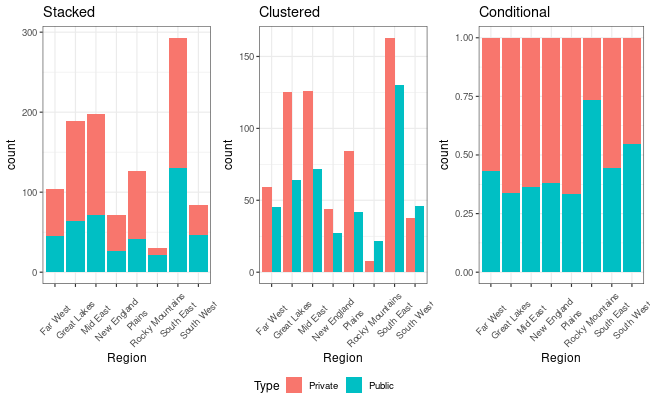
\includegraphics[scale=0.5]{bar_types.png}
\end{center}
\end{frame}

\begin{frame}{Stacked Bar Example}

\begin{center}
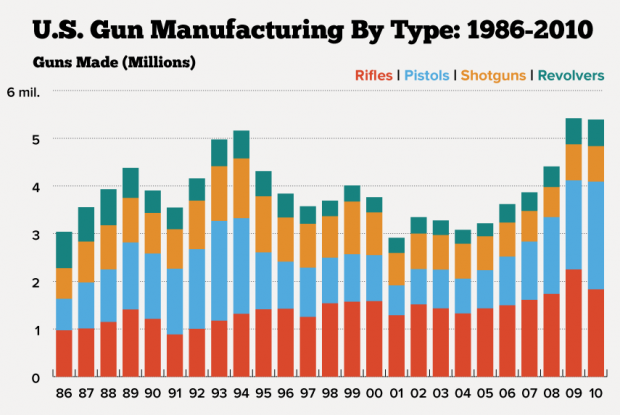
\includegraphics[scale=0.4]{stacked_bar_example.png}
{\tiny https://stackoverflow.com/questions/64267754/plotting-a-time-series-stacked-bar-chart}
\end{center}

\end{frame}


\begin{frame}{Descriptive Statistics -- Categorical Variables}

{\footnotesize
Univariate categorical variables are often presented in \textit{tables}
\begin{itemize}
	\item \textbf{Frequencies:} counts how many of each case belongs to a particular category
	\item \textbf{Proportions:} fractions based upon frequencies, also called \textit{relative frequencies}
\end{itemize}
}

\vspace{3mm}

\begin{columns}

  \begin{column}{0.45\textwidth}
 {\small
Frequency table:
% latex table generated in R 4.3.2 by xtable 1.8-4 package
% Sat Feb  3 13:19:35 2024
\begin{table}[ht]
\centering
\begin{tabular}{rr}
  \hline
 & Frequency \\ 
  \hline
Private & 647 \\ 
  Public & 448 \\ 
   \hline
\end{tabular}
\end{table}

Table of proportions:

% latex table generated in R 4.3.2 by xtable 1.8-4 package
% Sat Feb  3 13:20:48 2024
\begin{table}[ht]
\centering
\begin{tabular}{rr}
  \hline
 & Proportion \\ 
  \hline
Private & 0.591 \\ 
  Public & 0.409 \\ 
   \hline
\end{tabular}
\end{table}
}
  \end{column}
  \begin{column}{0.45\textwidth}
\begin{center}
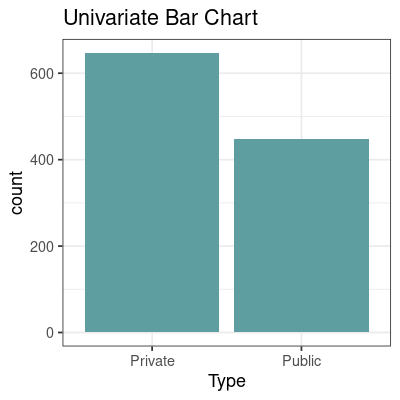
\includegraphics[scale=0.35]{univariate_bar.png}
\end{center}
  \end{column}

\end{columns}

\end{frame}

\begin{frame}{Bivariate Bar Charts}

Just as we did when looking at graphical summaries, we tend to designate variables as being either \textit{explanatory} or \textit{response} variables \vspace{4mm}

Again, this is \textbf{not} causal \vspace{4mm}

We tend to think of these relationships \textit{conditionally} when discussing categorical variables, a term we will return to shortly

\end{frame}

\begin{frame}{Descriptive Statistics -- Categorical Variables}


\begin{columns}

  \begin{column}{0.45\textwidth}
  
  Two-way frequency table:
  
\begin{table}[ht]
\centering
\begin{tabular}{rrr}
  \hline
 & Small & Large \\ 
  \hline
Private & 378 & 269 \\ 
  Public &  53 & 395 \\ 
   \hline
\end{tabular}
\end{table}
  \end{column}
  \begin{column}{0.45\textwidth}
\begin{center}
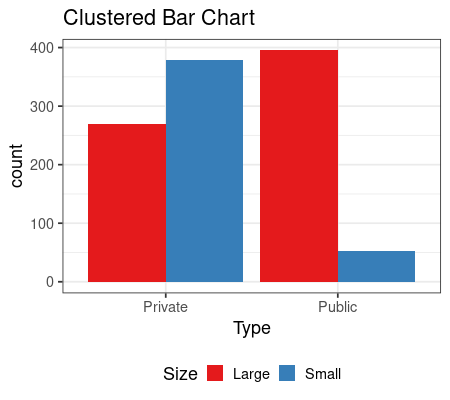
\includegraphics[scale=0.35]{bivariate_cluster.png}
\end{center}
  \end{column}

\end{columns}

\end{frame}



\begin{frame}{Descriptive Statistics -- Categorical Variables}
Often these tables include margin sums as well
\vspace{2mm}

\begin{columns}

  \begin{column}{0.45\textwidth}
  % latex table generated in R 4.4.1 by xtable 1.8-4 package
% Tue Sep 10 10:50:28 2024
\begin{table}[ht]
\centering
\begin{tabular}{rrr|c}
  \hline
 & Small & Large & Sum \\ 
  \hline
Private & 378 & 269 & 647 \\ 
  Public & 53 & 395 & 448 \\ \hline 
  Sum & 431 & 664 & 1095 \\ 
   \hline
\end{tabular}
\end{table}
  \end{column}
  \begin{column}{0.45\textwidth}
\begin{center}
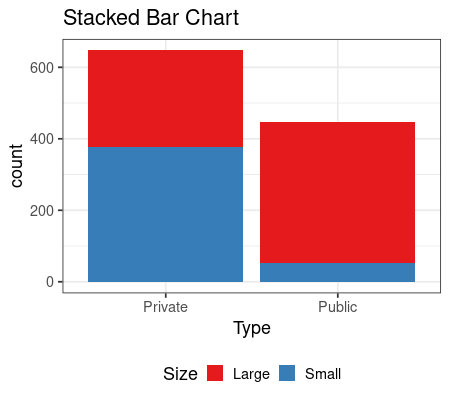
\includegraphics[scale=0.35]{bivariate_stack.png}
\end{center}
  \end{column}

\end{columns}
\end{frame}





\begin{frame}{Descriptive Statistics -- Categorical Variables}
Two-way table of proportions

% latex table generated in R 4.4.1 by xtable 1.8-4 package
% Tue Sep 10 10:51:45 2024
\begin{table}[ht]
\centering
\begin{tabular}{rrr}
  \hline
 & Small & Large \\ 
  \hline
Private & 0.3452 & 0.2457 \\ 
  Public & 0.0484 & 0.3607 \\  
   \hline
\end{tabular}
\end{table}


\textit{``36\% of all schools are large public schools"}
\end{frame}

\begin{frame}{Conditional Statistics}
A \textbf{conditional statistic} is a statistic derived from one or more variables for all observations sharing a value of another variable \vspace{2mm}
\begin{itemize}
	\item ``What is the relationship between admission rate and median ACT \textit{given} that the school is private"
	\item ``What is the predicted weight of an individual \textit{given} that they are 6ft tall"
	\item ``What is the proportion of public schools \textit{given} that we are looking at the Plains region"
\end{itemize}
\vspace{4mm}
Note that we typically condition on the \textit{explanatory} variable
\end{frame}


\begin{frame}{Descriptive Statistics -- Row Proportions}

\begin{columns}

  \begin{column}{0.45\textwidth}

{\small

\textit{``88\% of public schools are considered large"} \vspace{2mm}

\textit{``Given that a school is a public school, 88\% of them are considered large"} \vspace{2mm}
}  
  
% latex table generated in R 4.4.1 by xtable 1.8-4 package
% Tue Sep 10 10:56:53 2024
\begin{table}[ht]
\centering
\begin{tabular}{rrr}
  \hline
 & Small & Large \\ 
  \hline
Private & 0.5842 & 0.4158 \\ 
  Public & 0.1183 & 0.8817 \\ 
   \hline
\end{tabular}
\end{table}
  \end{column}
  \begin{column}{0.45\textwidth}
\begin{center}
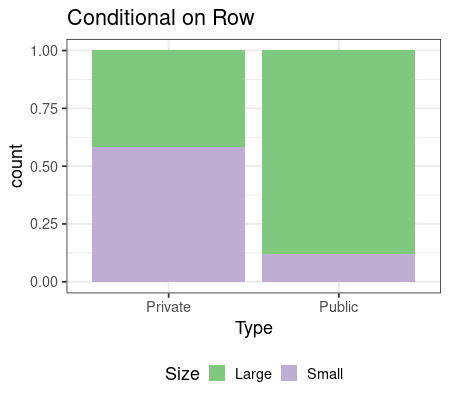
\includegraphics[scale=0.35]{bivariate_row.png}
\end{center}
  \end{column}

\end{columns}

\end{frame}




\begin{frame}{Descriptive Statistics -- Column Proportions}




\begin{columns}

  \begin{column}{0.45\textwidth}
 {\small \textit{``12\% of small colleges are public"}} \vspace{2mm}
% latex table generated in R 4.4.1 by xtable 1.8-4 package
% Tue Sep 10 10:57:46 2024
\begin{table}[ht]
\centering
\begin{tabular}{rrr}
  \hline
 & Small & Large \\ 
  \hline
Private & 0.8770 & 0.4051 \\ 
  Public & 0.1230 & 0.5949 \\ 
   \hline
\end{tabular}
\end{table}
  \end{column}
  \begin{column}{0.45\textwidth}
\begin{center}
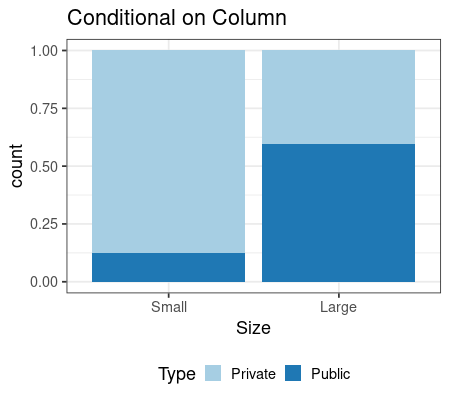
\includegraphics[scale=0.35]{bivariate_col.png}
\end{center}
  \end{column}

\end{columns}

\end{frame}


\begin{frame}{Example}
The two-way table below describes the survival of crew members and first class passengers aboard the Titanic

\begin{table}[ht]
\centering
\begin{tabular}{rrr}
  \hline
 & Survived & Died \\ 
  \hline
Crew & 212 & 673 \\ 
  First Class & 203 & 122 \\ 
   \hline
\end{tabular}
\end{table}

\begin{enumerate}
	\item Given that an individual survived, is it more likely that they were a crew member or a passenger in first class?
	\item Given that an individual was a crew member, is it more likely that they survived or died?
	\item Which group was more likely to survive the shipwreck?
\end{enumerate}
\end{frame}


\begin{frame}{Summary}

\begin{itemize}
\item Types of charts
\begin{itemize}
\item Stacked
\item Clustered
\item Conditional
\end{itemize}
\item Types of Tables
\begin{itemize}
\item One and two-way tables
\item Frequency and proportions
\item Which associated with which plots?
\end{itemize}
\item Association for categorical variables
\end{itemize}


\end{frame}


%%%%%%%%%%%%%%%%

%\begin{frame}
%\begin{columns}
%
%  \begin{column}{0.45\textwidth}
%%
%  \end{column}
%  \begin{column}{0.45\textwidth}
%%
%  \end{column}
%
%\end{columns}
%\end{frame}


\end{document}